\documentclass[preprint,11pt]{elsarticle}
%\documentclass[5p,times]{elsarticle}

\usepackage{hyperref}
\bibliographystyle{elsarticle-num}
\usepackage{balance}
\usepackage{multicol}
\usepackage{multirow}
\usepackage{tabularx}
\usepackage{amsmath}
\usepackage{float}
%\usepackage{lineno}
%\linenumbers
\usepackage{soul}
\usepackage{makecell}
\usepackage{color}
\usepackage{booktabs}

\hyphenpenalty=5000
\tolerance=1000

\graphicspath{{figures/}}
\renewcommand{\figurename}{{\bf Fig.}}

\begin{document}

\begin{frontmatter}

\title{Automated data processing pipeline and science data center for STIX}
\author{Hualin Xiao, Shane,Laslo, S\"am Krucker,  Ewan,  Gordon,Adrea,  Other STIX collaborators}
%\author[fhnw]{Hualin Xiao}
%\ead{hualin.xiao@fhnw.ch}

%\author[fhnw]{S{\"a}m Krucker}


\address[fhnw]{University of Applied Sciences and Arts Northwestern Switzerland (FHNW), 5200 Windisch, Switzerland}
\begin{abstract}
 The
Spectrometer/Telescope for Imaging X-rays (STIX) instrument onboard the Solar Orbiter mission launched
on February 10th 2020 promises advances in the study of solar flares of various sizes. It is capable of measuring
X-ray spectra from 4 to 150 keV with 1 keV resolution binned into 32 energy bins before downlinking
(KRUCKER et al., 2020).

\end{abstract}

 

\begin{keyword}
STIX; Data centre;
\end{keyword}
\end{frontmatter}

\section{Introduction}
Solar Orbiter
SOLO is a deep space mission study the Sun from close up (~1/3 AU) and from out of the ecliptic.

STIX
STIX is a hard X-ray imaging spectrometer which covers the energy range from 4 to 150 keV with 1 keV energy resolution. STIX uses a Fourier-transform imaging technique and provides an image to provide imaging on angular scales from 7 to 18 arcsec. For more detailed description of the instrument see the instrument paper [Krucker2020].


Bulk Processing via Parallel computing (BULPP) is a Technology Development 
Element activity that will respond to the need to perform large data 
reprocessing or reformatting to apply refined or evolved algorithms and data 
formats, and to improve data exploitation considering advanced techniques 
suitable for handling very large data quantities in limited time, e.g., by 
making use of the same auxiliary data for all the scenes or benefiting from a 
continuous information flow of the satellite data take. A proven possibility 
for improving the processing speed is to take advantage of the massive 
parallelization capabilities of Graphical Processing Units (GPUs). This 
parallelization is achieved with hundreds or thousands of processing cores 
that are able to work concurrently.As such the expected output of BULPP should 
be a modular bulk processing framework for EO payload data processing, based 
on a parallel (GPU) computing approach considering the overall end-to-end 
process, from the input data repository, often containing the lowest level 
data together with the auxiliary data needed for the processing, the 
scientific algorithms used in the current implementation, up to the output 
repository which will include reprocessed data and their metadata.The bulk 
processing framework shall be applicable to a variety of EO satellite missions 
and products, benefitting from commonalities, frequent usage, scalability and 
portability onto current (and future) state-of-the-art parallel processing 
technologies. This usually implies not only a change in the physical 
architecture,but also a full re-thinking, re-designing and re-writing of the 
software code.The envisaged bulk processing framework shall aim atextending 
the portfolio of parallelised (and parallelisable) algorithms, increasing the 
portability across different HW infrastructures, allowing data intensive 
processing close to the data storage, thus reducing the demands on network 
bandwidth and data transfer.
 
 
 STIX plays an important role in enabling Solar Orbiter to achieve one of its major science
goals: understanding the acceleration of electrons at the Sun and their transport into
interplanetary space. Specifically, the X-ray measurements made with STIX determine the
intensity, spectrum, timing, and location of accelerated electrons near the Sun. These
escaping electrons can then be tracked into the inner heliosphere through their type-III radio
emission, observed by RPW (the Radio and Plasma Waves instrument), and detected in situ
by STE (the SupraThermal Electron sensor) of the Energetic Particle Detector (EPD) suite,
to provide direct tracing of the magnetic structure, field line length, and connectivity. In this
way, STIX, together with RPW and STE, are able to magnetically link the heliospheric in situ
observations back to regions at the Sun where the electrons are accelerated.


\section{X-ray spectrometer and imager}

Data reception
Data parsing 
Database
Calibration automated processing
Online web viewers

Housekeeping data 
Quicklook data
Science data
Configuration database
Solar flare list
\section{operation tools}
operation request builder
flare detection


User science data requests
\section{level 0 data struction}
copy manual,
tree like, 
json formats
name, raw value, eng value, children
look-up table, to know description

estimat mongodb benchmark
Mongodb benchmark,
key value, index, performance


The connectivity tool can contribute to the prioritisation of data
downlink for instruments with internal memories (PHI, EUI,
STIX) and selective downlink for EPD and RPW, by helping the
instrument teams to make decisions on what datasets have higher
scientific importance and are therefore worth being downlinked
in priority. These could correspond to, for example, flare source
(RS) data connected to an event that has been measured IS or
vice versa, or an IS burst mode dataset that is probably linked to
a region that has been observed by RS high resolution imagers.
Once data have been acquired by Solar Orbiter, the LLD data
can be used to improve and/or validate the connectivity diagnos-
tic between a solar feature or event and its impact at the S/C
position. For example, STIX-LLD and EUI-LLD will provide
cross-checks for the occurrence of flare and CME activity in the
low corona, that can be used to flag events registered in the EPD-
LLD SEPs IS data. By combining both the information provided
by the connectivity forecast and the features seen in LLD, instru-
ment teams can make an informed decision on which data to
select from onboard storage.
As discussed in Sects. 5.2.2 and 5.4, LLD data will also pro-
vide invaluable real-time diagnostics that will help evaluating
(and even improving) the quality of the estimated connectivity.
For instance PAS-LLD data measurements can be used to pro-
vide the actual solar wind speed measured at Solar Orbiter (and
hence constraint the shape of the Parker spiral), and HIS-LLD
will guide the operators about the compositional and dynamical
properties of the plasma (and hence help disambiguate between
different candidate sources at the solar surface). PHI-LLD will
furthermore be used to improve the coronal magnetic field recon-
structions used for estimating connectivity across the corona.
Metis-LLD and Solar OrbiterHI-LLD can be used to derive the
position of streamers, to estimate CME trajectories, and to mea-
sure the wind speed acceleration and propagation profiles above
the visible limbs. Even though phenomena that propagate along
the limbs are not expected to affect directly the S/C, these obser-
vations will provide precious constraints for models that nowcast
the state of the eastern limb and eventually to suggest correc-
tions before these streams reach the S/C position (due to solar
rotation). In the same way, west limb information will provide
additional tests for models that may have been used to predict
the state of the solar plasma measured by the S/C a few days in
advance


\section{FITS data products}

The latest level 1 FITS io from Shane has been integrated into the data processing pipeline on pub023 server.

I have recreated fits products for all old telemetry data with the upgraded sw.

The L1 fits files  created by this pipeline have a different data level:  L1A ('A' here means  prerelease/alpha version).

The idea behind L1A data sets is to allow for quicker access to STIX data in the fits format instead of grabbing  data from plots or using json requests,

for operations,  debugging  etc.

The L1A data sets can be generated within a few minutes after the arrival of a new raw telemetry file.

The differences between L1A and L1 available in Shane's ftp include:

1.  Two different L1A data files may have duplicated data

2.  L1A data sets are still created for incomplete packets  (L1 checks for data completeness)

3.  SPICE kernel data for telemetry files always arrives  after one or two days later.

    So  there may be a sub-second difference between the UTC time in fits files (same to times on web pages)

   and the real time.

    Shane's formal L1 release can avoid this issue if they are produced on a later date.

4. L1A contains housekeeping data


\section{Data flow and data levels at STIX data center}
\begin{figure*}[!htb]
\begin{center}
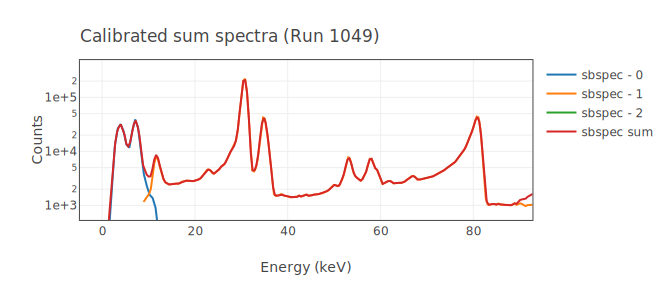
\includegraphics[width=0.9\textwidth]{calibration-example.pdf}
\caption{Data flow and data levels at the PSI POLAR data center. }
\label{fig:ch1}
\end{center}
\end{figure*}
\begin{figure*}[!htb]
\begin{center}
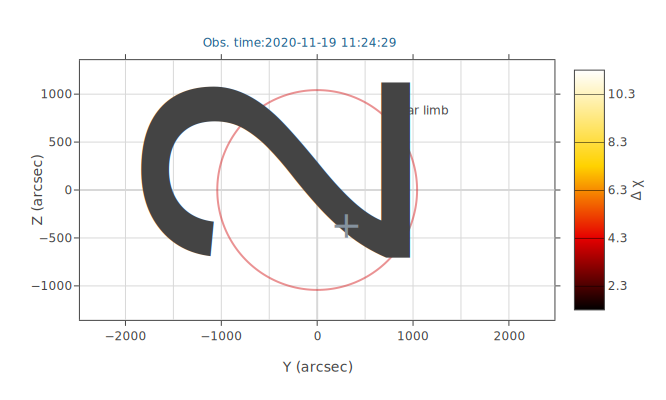
\includegraphics[width=0.7\textwidth]{cfl.pdf}
\caption{Data flow and data levels at the PSI POLAR data center. }
\label{fig:cfl}
\end{center}
\end{figure*}

\begin{figure*}[!htb]
\begin{center}
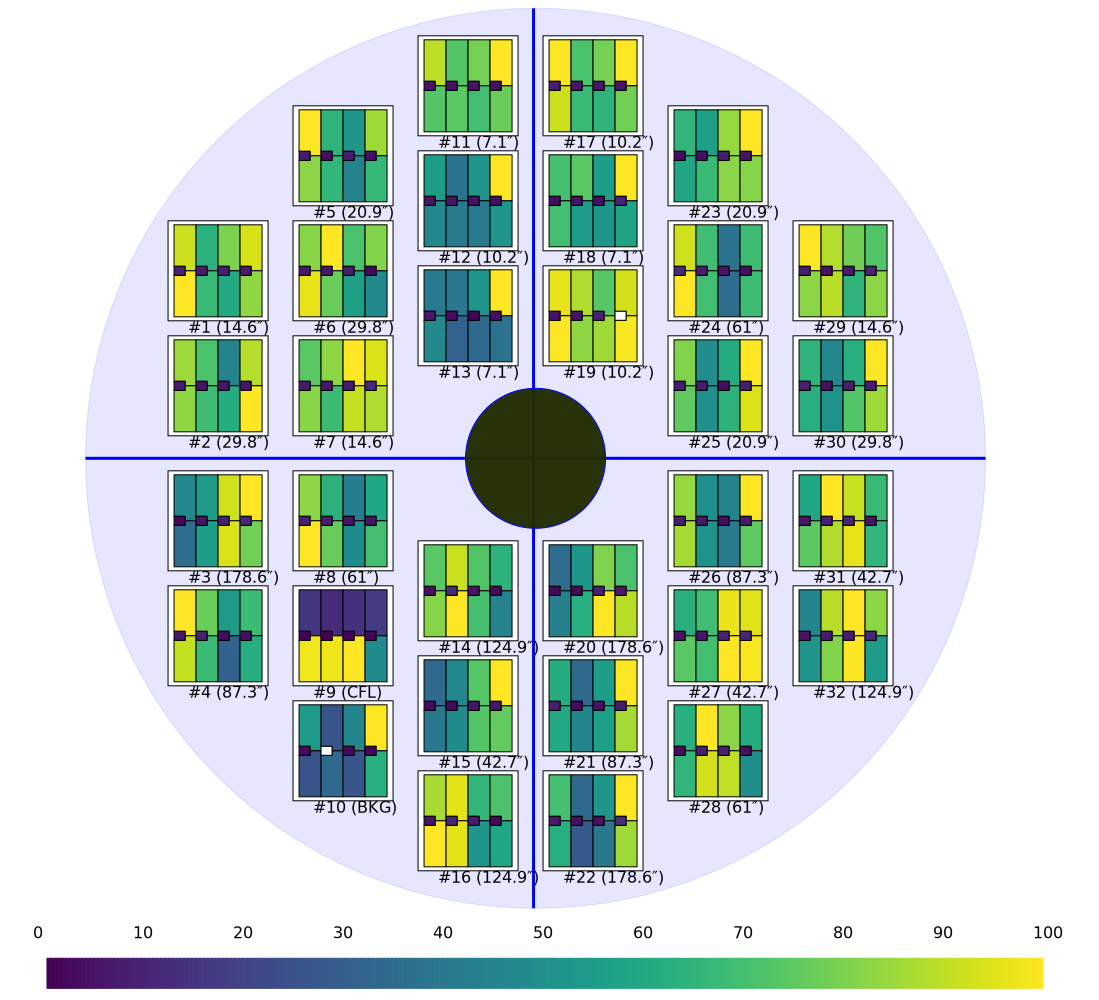
\includegraphics[width=0.7\textwidth]{l1-det-view.pdf}
\caption{Data flow and data levels at the PSI POLAR data center. }
\label{fig:det-view}
\end{center}
\end{figure*}


\begin{figure*}[!htb]
\begin{center}
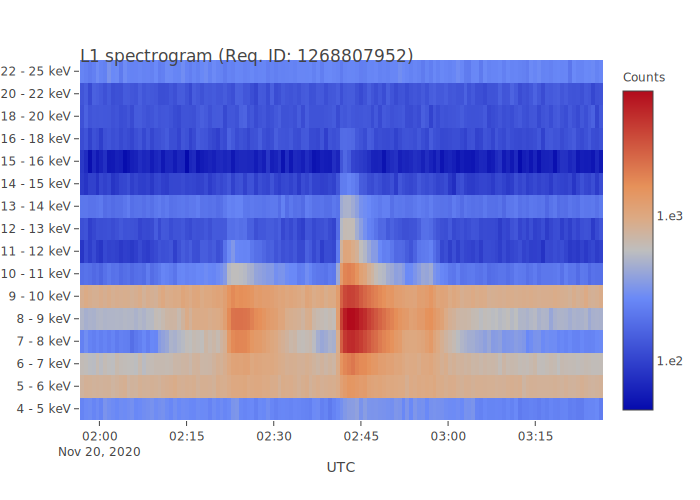
\includegraphics[width=0.7\textwidth]{l1-spectrogram.pdf}
\caption{Data flow and data levels at the PSI POLAR data center. }
\label{fig:det-view}
\end{center}
\end{figure*}

\section{calibration processing pipeline}

In the STIX instrument, a Ba134 radioactive source is placed at the front of each detector. The total activity of the radioactive source is approximately 4000 Ba.
When the radioactive source decays, gamma rays are generated. These gamma rays can form peaks in the energy spectrum of the detector.
The corresponding energy is known, and the corresponding relationship between ADC and real energy can be calibrated through the position of the peak in the energy spectrum, that is, the calibration coefficient. The figure below is a typical Ba133 gamma-ray energy spectrum measured by STIX CdTe detector. There are three obvious peaks in the energy spectrum, and they correspond to three energies of 30 keV, 35 keV and 81 keV. There are many ways to determine the position of each peak, you can use the ECC method, or use the Gaussian function to fit the left part of the peak.

\subsection{Generation of fits file}

\section{ APIs}
\subsection{Fits api}
\subsection{configuration apis}
\section{Web data visualization tools}
Think about a tall building in your neighborhood. If given the option, would it be better to add more floors in this building or create a new building entirely for more residents?

This is the problem for SQL and NoSQL databases. SQL databases are vertically scalable. This means that the load on a single server can be increased by increasing things like RAM, CPU, or SSD. (More floors can be added to this building). On the other hand, NoSQL databases are horizontally scalable. This means that more traffic can be handled by sharding, or adding more servers in your NoSQL database. (More buildings can be added to the neighborhood).

In the long run, it is better to add more buildings than floors as that is more stable (Less chance of creating a Leaning Tower of Pisa!!!). Thus, NoSQL can ultimately become larger and more powerful, making NoSQL databases the preferred choice for large or ever-changing data sets.

3. Schema Design
A schema refers to the blueprint of a database i.e how the data is organized. The schema of an SQL database and a NoSQL database is markedly different. Let’s use a joke to better understand this.
\end{document}
